
\begin{frame}
\frametitle{Les 6: Het dienbladenprobleem {\small (vervolg)}}
\framesubtitle{Didactische wenken}

\begin{enumerate}
	\item Onderwijsleergesprek
	\begin{itemize}
	\item Doel van deze les en de opdracht laten aanvoelen en uitleggen
\end{itemize}
	
	\item In groepjes werken
	\begin{itemize}
	\item A.d.h.v. een bundeltje met vragen en opdrachten iets bewijzen waarbij ze het stappenplan kunnen volgen
	\item M.b.v. een (zelfgemaakte) figuur het bewijs visueel maken
	\item Experimenteren, tekenen en berekenen
	% Leerkracht helpt waar nodig en loopt rond!!
\end{itemize}

  \item Onderwijsleergesprek
  \begin{itemize}
  \item Moeilijkheden en problemen in het bewijs samen overlopen
  \item Eventueel nog enkele ingewikkeldere configuraties berekenen
	\item Resultaten in de tabel samenleggen.
\end{itemize}

  \item Klasgesprek
  \begin{itemize}
	  \item Opmerkelijke zaken bespreken
	  \item Conclusies trekken
  \end{itemize}
\end{enumerate}
\end{frame}



%\begin{frame}
%\frametitle{Tweedimensionale stapelproblemen}
%\framesubtitle{Dienbladenprobleem}

%\begin{block}{Opdracht}
%Geef voorbeelden van configuraties met 4 munten die je niet verder kan verschuiven.
%\end{block}
%\pause

%\begin{figure}[h]
%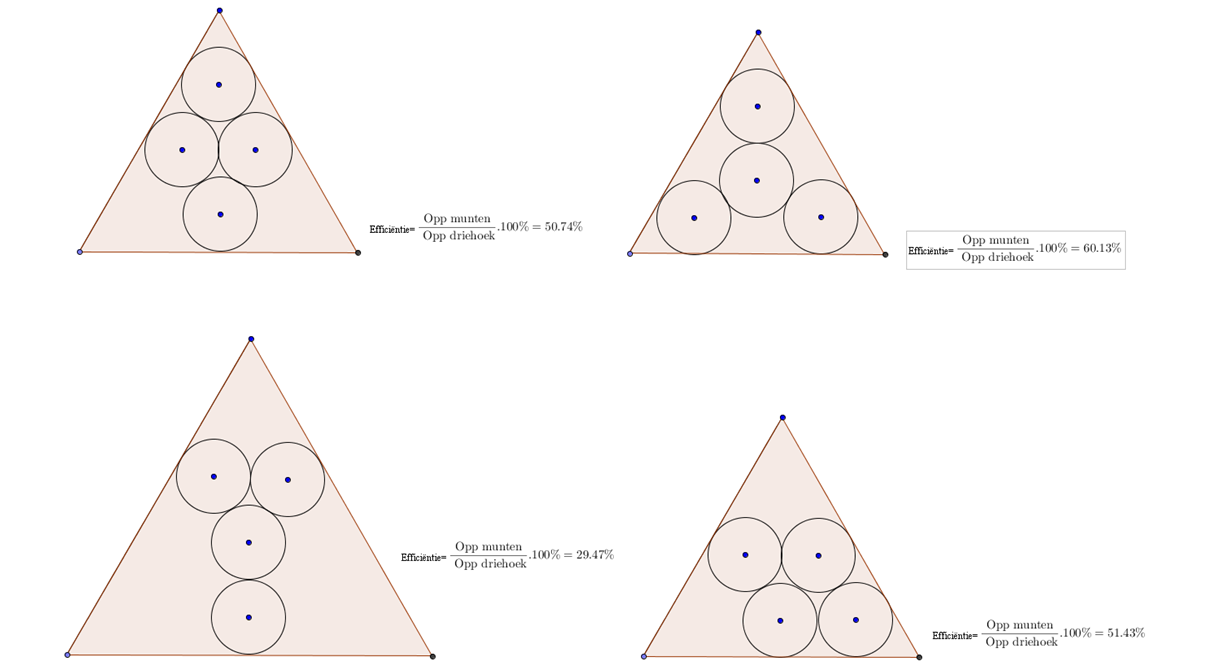
\includegraphics[height=4cm]{figuur4munten}
 % \caption{Configuraties met 4 munten in een driehoekig dienblad, die je niet verder kunt duwen, met verschillende effici�nties.}  
%\end{figure}
%\end{frame}



%\begin{frame}
%\frametitle{Tweedimensionale stapelproblemen}
%\framesubtitle{Dienbladenprobleem}

%\begin{block}{Vraag}
%Welke configuratie is de meest effici�nte?
%\end{block}
%\pause
%\begin{figure}[ht]
 % \centering
  %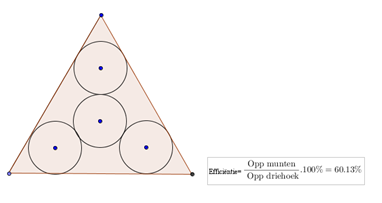
\includegraphics[height=3cm]{fig2}
  %\caption{Meest effici�nte configuratie met 4 munten in een driehoekig dienblad.}
  %\label{fig:efficientsteconfig}
%\end{figure}
%\pause
%\begin{block}{Opdracht}
%Bewijs dit!
%\end{block}


%\end{frame}


\begin{frame}
\frametitle{Les 6: Het dienbladenprobleem {\small (vervolg)}}
\framesubtitle{Didactische wenken}

\begin{enumerate}
	\item Onderwijsleergesprek
	\begin{itemize}
	\item Doel van deze les en de opdracht laten aanvoelen en uitleggen
\end{itemize}
	
	\item In groepjes werken
	\begin{itemize}
	\item A.d.h.v. een bundeltje met vragen en opdrachten iets bewijzen waarbij ze het stappenplan kunnen volgen
	\item M.b.v. een (zelfgemaakte) figuur het bewijs visueel maken
	\item Experimenteren, tekenen en berekenen
	% Leerkracht helpt waar nodig en loopt rond!!
\end{itemize}

  \item Onderwijsleergesprek
  \begin{itemize}
  \item Moeilijkheden en problemen in het bewijs samen overlopen
  \item Eventueel nog enkele ingewikkeldere configuraties berekenen
	\item Resultaten in de tabel samenleggen.
\end{itemize}

  \item Klasgesprek
  \begin{itemize}
	  \item Opmerkelijke zaken bespreken
	  \item Conclusies trekken
  \end{itemize}
\end{enumerate}
\end{frame}



\begin{frame}
\frametitle{Tweedimensionale stapelproblemen}
\framesubtitle{Dienbladenprobleem: Conclusie}



\begin{table}[h]
\centering
\small
\begin{tabular}{l||c|c|c|c}
Aantal / vorm & cirkelvormig & driehoekig & rechthoekig& zeshoekig\\\hline\hline
1&  100\% & 60,46\% & 78,54\%&90,69\%\\\hline
2& 50\%& 48,60\% & 78,54\%& 52,09\% \\\hline
3&64,62\%& 72,90\%  & 78,54\%& 68,02\%\\\hline
4&67,13\%&60,46\%&78,54\%&66,93\%\\\hline
5&68,52\%& 65,11\%  & 78,54\%& 62,14\%\\\hline
6&67,13\%&77,41\%&78,54\%&65,10\%\\\hline
7&77,78\%& 63,71\%  & 78,54\%& 85,05\%\\\hline
8&72,42\%&64,02\%&78,54\%&69,03\%\\\hline
9&67,57\%&72,02\%&78,54\%&66,03\%\\\hline
10&66,94\%&79,06\%&78,54\%& 71,13\%\\\hline
11&71,45\%& 64,40\%  & 79,06\%& 64,79 \%\\\hline
12&73,58\%&65,75\%&78,54\%&75,99\%\\\hline
13&72,45\%& 71,77 \%  & 78,54\%& 70,20 \%
\end{tabular}
\caption{\scriptsize De effici�ntie van de dienbladen bij een bepaalde hoeveelheid glazen of blikjes.}
\label{}
\end{table}



\end{frame}


\begin{frame}
\frametitle{Tweedimensionale stapelproblemen}
\framesubtitle{Dienbladenprobleem: Conclusie}



\begin{table}[h]
\centering
\small
\begin{tabular}{l||c|c|c|c}
Aantal / vorm & cirkelvormig & driehoekig & rechthoekig& zeshoekig\\\hline\hline
1& \cellcolor[rgb]{0.6,0.6,0.6} 100\% & 60,46\% & 78,54\%&90,69\%\\\hline
2& 50\%& 48,60\% & \cellcolor[rgb]{0.6,0.6,0.6}78,54\%& 52,09\% \\\hline
3&64,62\%& 72,90\% \cellcolor[rgb]{0.6,0.6,0.6} & 78,54\%& 68,02\%\\\hline
4&67,13\%&60,46\%&\cellcolor[rgb]{0.6,0.6,0.6}78,54\%&66,93\%\\\hline
5&68,52\%& 65,11\%  &\cellcolor[rgb]{0.6,0.6,0.6} 78,54\%& 62,14\%\\\hline
6&67,13\%&77,41\%&\cellcolor[rgb]{0.6,0.6,0.6}78,54\%&65,10\%\\\hline
7&77,78\%& 63,71\%  & 78,54\%& \cellcolor[rgb]{0.6,0.6,0.6} 85,05\%\\\hline
8&72,42\%&64,02\%&\cellcolor[rgb]{0.6,0.6,0.6}78,54\%&69,03\%\\\hline
9&67,57\%&72,02\%&\cellcolor[rgb]{0.6,0.6,0.6}78,54\%&66,03\%\\\hline
10&66,94\%&\cellcolor[rgb]{0.6,0.6,0.6}79,06&78,54\%& 71,13\%\\\hline
11&71,45\%& 64,40\%  & \cellcolor[rgb]{0.6,0.6,0.6}79,06\%& 64,79 \%\\\hline
12&73,58\%&65,75\%&\cellcolor[rgb]{0.6,0.6,0.6}78,54\%&75,99\%\\\hline
13&72,45\%& 71,77 \%  &\cellcolor[rgb]{0.6,0.6,0.6} 78,54\%& 70,20 \%
\end{tabular}
\caption{\scriptsize De effici�ntie van de dienbladen bij een bepaalde hoeveelheid glazen of blikjes.}
\label{}
\end{table}



\end{frame}
